\sect{Turingmaschinen (TM)}

Eine TM ist informell ein endlicher Automat, ergänzt mit einem Lese-/Schreibkopf und ein unendliches Band von Zellen mit Leerzeichen.
Die Eingabe steht am Anfang auf dem Band.

Eine \textbf{deterministische TM} ist ein 7-Tupel $M = (Q, \Sigma, \Gamma, \delta, q_0, \textvisiblespace, F)$ mit
\begin{itemize}
    \item \emph{endlichen} Menge von Zuständen $Q = \{q_0, \dots, q_n\}$
    \item Eingabealphabet $\Sigma = \{a_1, \dots, a_m\}$
    \item Übergangsfunktion $\delta: Q \times \Gamma \rightarrow Q \times \Gamma \times D, D =\{L,R\}$
    \item Startzustand $q_0 \in Q$
    \item Menge von akzeptierenden Zuständen $F \subseteq Q$
    \item Bandalphabet $\Gamma$ (endliche Menge von Symbolen) und $\Sigma \subset \Gamma$
    \item Leerzeichen \textvisiblespace, mit $\textvisiblespace \in \Gamma$ und $\textvisiblespace \notin \Sigma$
\end{itemize}

Die Übergangsfunktion $\delta$ bildet das 2-Tupel $(q, X)$ auf das Tripel $(p, Y, D)$ ab
\begin{itemize}
    \item $q,p \in Q$ und $X, Y \in \Gamma$
    \item $D$ ist die Bewegung des Lese-/Schreibkopfes über dem Band und nimmt die Werte $L$ (Links) oder $R$ (Rechts) an.
\end{itemize}

% TODO: TM Beispiel

\ssect{Vergleich Übergangsfunktion}

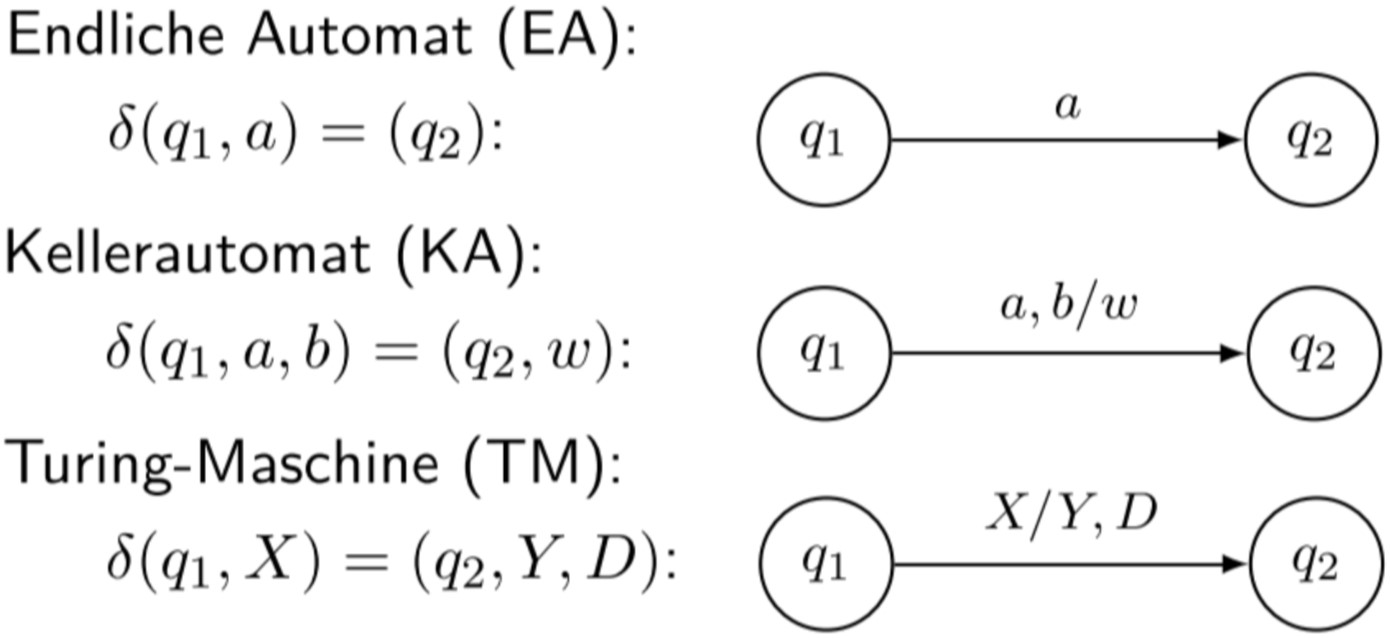
\includegraphics[scale=0.18]{vergleich}%